\documentclass[a4paper]{article}

\usepackage[utf8]{inputenc}
\usepackage[T1]{fontenc}
\usepackage{amsmath, amssymb, physics, braket, graphicx, wrapfig}

\newcommand{\N}[0]{\mathcal{N}}

\newcommand{\Ha}[0]{\mathcal{H}}

\newcommand{\com}[2]{[#1,#2]}
\newcommand{\acom}[2]{\{#1,#2\}}

\newcommand{\da}[0]{^{\dagger}}

\title{Supersymmetry - Introduction}
\author{Ivo A. Maceira}

\begin{document}
\maketitle
\footnote{Introduction to Supersymmetry, Lykken 1996}Most general spacetime symmetry algebra of QFTs assuming locality, causality, positive energy, \dots
\begin{itemize}
	\item using
		$
		\com{\cdot}{\cdot}:
		$

	\item[] Poincaré Lie Algebra:\\
	$P_0 = \Ha, P_i, J_i, K_i$

	\item using
		$
		\com{\cdot}{\cdot}
		$
		and
		$
		\acom{\cdot}{\cdot}:
		$

	\item[] SuperPoincaré Graded Lie Algebra of grade $\N$:\\
		Poincaré + SUSY generators
		$
		\underbrace{R_1^-,R_1^+,R_2^-,R_2^+}_{\N = 1},\dots
		$

\end{itemize}

Properties:
\begin{equation}
	R_i^- = R_i,\quad R_i^+ = R_i\da
\end{equation}

\begin{align}
	\com{P_{\mu}}{R^{\pm}_i} &= 0,\\
	\com{J_z}{R_1^{\pm}} &= \pm\frac{1}{2} R_1^{\pm},\\
	\acom{R_i^{\pm}}{R_j^{\pm}} &= 0 \implies (R_i^{\pm})^2 = 0, \\
	\acom{R_1^+}{R_1^-} &= \Ha - P_z, \\
	\acom{R_2^+}{R_2^-} &= \Ha + P_z \\
\end{align}

\begin{align}
	\implies 2\Ha &= \acom{R_1^+}{R_1^-} + \acom{R_2^+}{R_2^-}, \\
	\text{if } P_z = 0: \Ha &= \acom{R_1^+}{R_1^-} \equiv \acom{R^+}{R^-}
\end{align}

Summary:
\begin{equation}
	\Ha = R\da R + R R\da,
\end{equation}

\begin{align}
	&R^2 = (R\da)^2 = 0,&\quad& \com{J_z}{\Ha} = 0, \\
	&\com{R^{\pm}}{\Ha} = 0,&\quad& \com{J_z}{R^{\pm}} = \pm \frac{1}{2} R^{\pm}\quad (J^{\pm}),
\end{align}

Consequences on Hilbert Space:

\begin{equation}
	\implies
	\begin{cases}
		J_z \ket{j} = j \ket{j}\\
		\Ha \ket{j} = E \ket{j}\\
	\end{cases}, \braket{j|j} = 1
\end{equation}

\begin{equation}
	\implies
	\begin{cases}
		R^{\pm} \ket{j} = c^{\pm} \ket{j \pm \frac{1}{2}} \\
		c^{\pm} \geq 0 \\
		\braket{j\pm \frac{1}{2}|j\pm \frac{1}{2}} = 1
	\end{cases},
\end{equation}

Assuming
$
R\ket{j} = 0,
$
then
\begin{align}
	\implies \text{either}
	&\begin{cases}
		R^{+} \ket{j} = 0\\
		E = 0
	\end{cases},\\
	\text{or}
	&\begin{cases}
		R^{+} \ket{j} = \sqrt{E} \ket{j + \frac{1}{2}}, E>0\\
		R \ket{j + \frac{1}{2}} = \sqrt{E} \ket{j}\\
		\Ha \ket{j + \frac{1}{2}} = E \ket{j + \frac{1}{2}}\\
	\end{cases}
\end{align}

For all $\ket{j}$:
\begin{align}
	\text{either } &R^{+} \ket{j} = 0,\\
	\text{or }     &R^{+} \ket{j} = \sqrt{E} \ket{j + \frac{1}{2}}, E>0
\end{align}

\begin{wrapfigure}{l}{0.33\textwidth}
	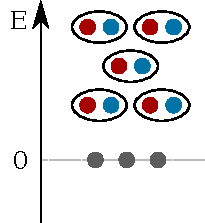
\includegraphics[width=0.33\textwidth]{Figures/Supersymmetric_spectrum.pdf}
	\caption{Supersymmetric spectrum. Positive energy states form duplets where the two states are related by the supersymmetric charge. Zero energy states are singlets. }
	\label{fig:Supersymmetric_spectrum}
\end{wrapfigure}

Summary:
\begin{align}
	E = 0 & \implies R^{\pm} \ket{j} = 0,\\
	E > 0 & \implies 
	\begin{cases}
		R^+ \ket{j} = \sqrt{E} \ket{j + \frac{1}{2}} \\
		R \ket{j + \frac{1}{2}} = \sqrt{E} \ket{j}
	\end{cases}.
\end{align}

Hermitian Operators $Q,\tilde{Q}$
\begin{align}
	Q &= R + R^+&\quad (J_x), \\
	\tilde{Q} &= i(R - R^+)&\quad (J_y).
\end{align}

\begin{equation}
	Q \left(\ket{j} \pm \ket{j \pm \frac{1}{2}}\right)  = \pm \sqrt{E} \left( \ket{j} \pm \ket{j \pm \frac{1}{2}} \right).
\end{equation}

Supersymmetry Breaking:
\begin{align}
	\frac{E_0}{N} = 0 &\implies Q_0 = 0 \implies \text{No S.B.} \\
	\frac{E_0}{N} > 0 &\implies Q_0 = \pm \sqrt{E_0} \implies \text{S.B.}
\end{align}

Witten Index - Count all states in Hilbert space with
\begin{itemize}
		\item integer spin: $(n_I)$
		\item half-integer spin: $(n_{HI})$
\end{itemize}

At least $|W| \equiv |n_I - n_{HI}|$ states have $E=0$.
Witten index of $N$ fermions Hilbert space is 0.
Check (Fendley, Schoutens 2003) for models with non-zero Witten index.

\footnote{Nicolai 1976}Lattice Supersymmetry:

\begin{itemize}
	\item bosons + fermions:
		\begin{equation}
			R^{+} = \sum_{i}^{} f_i\da b_i.
		\end{equation}
	\item fermions:
		\begin{equation}
			R^{+} = \sum_{i}^{} f_i.
		\end{equation}
		Only odd terms are allowed $\Leftrightarrow$ $\Ha$ is local.
	\item Majoranas:
		\begin{equation}
			Q = \sum_{i}^{} \gamma_i.
		\end{equation}
		If $Q \ket{F \text{ odd}} = \ket{F \text{ even}} \implies$
		\begin{equation}
			\begin{cases}
				Q \ket{\pm} = \pm \sqrt{E} \ket{\pm}\\
				\Ha \ket{\pm} = \pm E \ket{\pm}\\
			\end{cases}\footnote{Is it actually true? check!}
		\end{equation}
\end{itemize}

\end{document}
